% !TeX root = METOD.tex
\chapter{Термодинамика газа Ван-дер-Ваальса (ВдВ).}

\emph{Газом Ван-дер-Ваальса} называется модель реального газа, которая
описывается уравнением Ван-дер-Ваальса:
\begin{equation}
  \left ( P+\frac{a}{V^2}\right )(V-b) = RT.
\end{equation}
Это уравнение отличается от уравнения Менделеева-Клапейрона двумя
поправками:

$b$~---~поправка, учитывающая собственный объем молекул,

$\cfrac{a}{V^2}$~---~поправка, учитывающая внутреннее давление, определяемое притяжением молекул газа между собой.

В этой модели учитываются взаимодействие молекул между собой на расстоянии
и размеры молекул путем введения соответствующих поправок \emph{a} и
\emph{b}, поэтому часто говорят, что уравнение Ван-дер-Ваальса~---~это
простейшее уравнение состояния реального газа (см. главу \ref{equationOfState}).

Уравнение Ван-дер-Ваальса качественно правильно передает поведение
реальных газов даже при переходе их в жидкость. На рис. \ref{isotermsVDV} изображены
изотермы Ван-дер-Ваальса на диаграмме $(P, V)$.
\begin{wrapfigure}{r}{.5\textwidth}
  \centering
  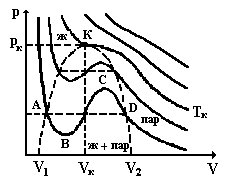
\includegraphics[width=.5\textwidth]{isotermsVDV.png}
  \caption{}
  \label{isotermsVDV}
\end{wrapfigure}
Эксперимент показывает, что изотермы Ван-дер-Ваальса качественно правильно передают зависимость $P(V)$, однако при объемах $V_1 < V < V_2$,
когда происходит переход из жидкого состояния в газообразное и наоборот,
давление не изменяется, т.е. экспериментальным данным соответствует
прямая AD, а не кривая ABCD. Точка К на графике, которая определяется
как точка перегиба критической изотермы (при $T =
T_k$), соответствует \emph{критическому состоянию} (см. главу \ref{equationOfState}).

Давление \emph{p\textsubscript{к}} и объем \emph{V\textsubscript{к}}
вещества в этом состоянии, называются соответственно \emph{критическим
давлением} и \emph{критическим объемом.}

\emph{В критическом состоянии исчезает различие между жидким и
парообразным состоянием вещества. Выше критической точки вещество может
находиться лишь в газообразном состоянии.}

\textbf{Контрольные вопросы.}

\begin{enumerate}
\def\labelenumi{\arabic{enumi}.}
\item Возможно ли реально осуществить состояния, соответствующие участкам
  AB, DC и CD изотермы Ван-дер-Ваальса? Как называются такие состояния?
  Чем они характеризуются?
\item Пользуясь основным уравнением термодинамики докажите правило
  Максвелла: на диаграмме (\emph{p, V}) (рис. \ref{isotermsVDV}) площади криволинейных
  треугольников, образующихся при пересечении изотермы Ван-дер-Ваальса
  экспериментальной прямой AD, одинаковы.
\item Чем объясняется зависимость внутренней энергии газа Ван-дер-Ваальса от
  объема?
\item Объясните, чем определяется различие в поведении идеального газа и
  газа Ван-дер-Ваальса при расширении их в пустоту.
\item В чем состоит эффект Джоуля-Томсона, и какой величиной он
  характеризуется? Является ли соответствующий процесс обратимым?
\item В каком случае эффект Джоуля-Томсона считается положительным, а в
  каком отрицательным? Что такое температура инверсии этого эффекта, и
  чему она равна?
\end{enumerate}

\textbf{Литература}

{[}1{]}. Гл. 1. § 6.

{[}2{]}. Гл. 8. § 30.

{[}3{]}. Гл. 7. § 5.

{[}4{]}. Гл. 8. §§ 97 - 105, Гл. 10. §§ 117, 119.

{[}5{]}. Гл. 6. §§ 54 - 62.

\textbf{Задачи}

\section{Найти работу, совершаемую одним молем газа ВдВ при
изотермическом расширении от объема \emph{V\textsubscript{1}} до
\emph{V\textsubscript{2}} . Известна температура газа и поправки ВдВ.}

\solving{}

Подставляя в общую формулу работы силы давления выражение для давления,
полученное из уравнения ВдВ, имеем:

\begin{equation}
  A = \int\limits_{V_1}^{V_2} PdV = \int\limits_{V_1}^{V_2} \left (  \frac{RT}{V-b} - \frac{a}{V^2}\right )dV = RTln\frac{V_2-b}{V_1-b} + \left ( \frac{a}{V_1} - \frac{a}{V_2}\right ).
\end{equation}

\section{Показать, что для газа ВдВ теплоемкость $C_V$ не зависит от объема V и,
следовательно, совпадает с изохорной теплоемкостью идеального газа
\emph{С\textsubscript{V} = (i / 2) R}.} Указание. Воспользоваться
результатом задачи \ref{ThermKalEq}.

\solving{}

Из определения и первого закона термодинамики следует, что изохорная
теплоемкость равна $C_V = \left ( \cfrac{\partial U}{\partial T} \right )_V$. Чтобы она не
зависела от объема, необходимо равенство нулю ее производной, т. е.
\begin{equation}
  \left ( \frac{\partial C_V}{\partial V} \right )_T = \frac{\partial^2 U}{\partial V \partial T} =0.
\end{equation}
Из дифференциальной связи термического и калорического уравнений
состояния (задача \ref{ThermKalEq}) следует:
\begin{eqnarray}
  \frac{\partial^2 U}{\partial V \partial T} = \frac{\partial^2 U}{\partial T \partial V} = \frac{\partial}{\partial T} \left ( \left (\frac{\partial U}{\partial V}\right )_T \right ) = \nonumber \\
  = T \left (\frac{\partial^2 P}{\partial T^2}\right )_V + \left (\frac{\partial P}{\partial T}\right )_V - \left (\frac{\partial P}{\partial T}\right )_V = T \left (\frac{\partial^2 P}{\partial T^2}\right )_V
\end{eqnarray}
Здесь использована независимость второй производной от порядка
дифференцирования.

Дифференцируя выражение для давления, полученное из уравнения ВдВ, по
температуре, получаем:
\begin{equation}
  P = \frac{RT}{V-b} - \frac{a}{V^2} \Rightarrow \left (\frac{\partial P}{\partial T} \right )_V = \frac{R}{V-b} \Rightarrow \left (\frac{\partial^2 P}{\partial T^2} \right )_V = 0.
\end{equation}
Таким образом мы видим, что изохорная теплоемкость $C_V$ для газа ВдВ не зависит от объема. Учитывая, что газ ВдВ является предельным случаем идеального газа при $V \rightarrow
0$, получаем значение изохорной теплоемкости газа ВдВ:
$C_V = (i/2) R$.

\section{Найти зависимость внутренней энергии газа ВдВ, считая, что
\emph{С\textsubscript{V}} не зависит от температуры.}

\solving{}

Полагая, что внутренняя энергия является функцией объема и температуры,
получаем выражение для ее полного дифференциала:
\begin{equation}
  dU = \left ( \frac{\partial U}{\partial V}\right )_TdV + \left ( \frac{\partial U}{\partial T}\right )_VdT.
\end{equation}
Производную внутренней энергии по объему легко найти, используя
дифференциальную связь уравнений состояния:
\begin{equation}
  \left ( \frac{\partial U}{\partial V}\right )_T = T\left ( \frac{\partial P}{\partial T}\right )_V - P = T\cdot\frac{R}{V-b} - \left (\frac{RT}{V-b}-\frac{a}{V^2} \right ) = \frac{a}{V^2}.
\end{equation}
Производная же по температуре представляет собой изохорную теплоемкость,
которую мы считаем не зависящей от температуры. С учетом этого для
дифференциала внутренней энергии получаем:
\begin{equation}
  dU = \frac{a}{V^2}dV + C_VdT.
\end{equation}
Интегрируя выражение (3), находим:
\begin{equation} \label{internalEnergyOfVDV}
  U = -\frac{a}{V} + C_VT.
\end{equation}
Второе слагаемое в формуле \ref{internalEnergyOfVDV} совпадает с выражением для внутренней
энергии идеального газа. Оно представляет собой суммарную кинетическую
энергию движения молекул. Первое же слагаемое учитывает потенциальную
энергию взаимодействия молекул между собой. В модели идеального газа
этим взаимодействием пренебрегают, поэтому соответствующее слагаемое в
выражении для внутренней энергии отсутствует.

\section{Найти изменение температуры газа ВдВ при адиабатическом
расширении в вакуум от объема \emph{V\textsubscript{1}} до
\emph{V\textsubscript{2}}.}

\solving{}

Из адиабатичности процесса и равенства нулю работы газа следует, что при
адиабатическом расширении в вакуум внутренняя энергия газа не
изменяется. (См. также задачу \ref{entropyOfVacuum}) Используя выражение для внутренней
энергии газа ВдВ, полученное в предыдущей задаче, получаем:
\begin{equation} \label{internalEnergyOfVacuum}
  \Delta U = C_V\Delta T -a \left (\frac{1}{V_2} - \frac{1}{V_1} \right ) = 0 \Rightarrow \Delta T = \frac{a}{C_V}\left (\frac{1}{V_2} - \frac{1}{V_1} \right ) < 0.
\end{equation}
Из формулы \ref{internalEnergyOfVacuum} видно, что газ ВдВ при адиабатическом расширении в вакуум
охлаждается.

\section{Вычислить энтропию газа Ван-дер-Ваальса.}

\solving{}

Из объединенного закона термодинамики для обратимых процессов имеем:
\begin{equation}
  dS = (\delta A + dU)/T.
\end{equation}
\emph{dS = (δA + dU) / T} . (1)

Отсюда, подставляя выражение для работы силы давления

\emph{δA = pdV} ,

где давление \emph{p} определяется из уравнения ВдВ : \emph{p = RT /
(V-b) - a / V\textsuperscript{2}} ,

а затем интегрируя, получаем:

%\includegraphics{media/image119.wmf}. (2)

54

Интегрируя выражение (2), находим:

%\includegraphics{media/image120.wmf} , (3)

где S\textsubscript{0} - некоторая постоянная.

\section{Найти теплоемкость газа ВдВ при постоянном давлении.}

\solving{}

Из определения теплоемкости следует:
%\includegraphics{media/image121.wmf}. (1)

Полагая, что внутренняя энергия является функцией объема и температуры
\emph{U = U( V, T)}, преобразуем первый закон термодинамики к виду:

%\includegraphics{media/image122.wmf}. (2)

Отсюда для теплоемкости \emph{С\textsubscript{p}} получаем:

%\includegraphics{media/image123.wmf} , (3)

где учтено выражение для изохорной теплоемкости
%\includegraphics{media/image124.wmf} .

Выражение (3) справедливо в общем случае для любого газа. В случае газа
ВдВ имеем: %\includegraphics{media/image125.wmf} . (4)

Учитывая, что %\includegraphics{media/image126.wmf} , (5)

из уравнения ВдВ находим:

%\includegraphics{media/image127.wmf}. (6)

Откуда получаем: %\includegraphics{media/image128.wmf}. (7)

55

Подставляя (4) и (7) в выражение (3) , имеем:

%\includegraphics{media/image129.wmf} . (8)

Учитывая, что \emph{b \textless\textless{} V}, и сохраняя только малые
величины первого порядка, получим:

%\includegraphics{media/image130.wmf} . (9)

Из формул (8) и (9) видно, что уравнение Майера оказывается справедливым
только для идеального газа. В общем случае неидеальных газов разность
теплоемкостей \emph{С\textsubscript{p} - C\textsubscript{V}} зависит от
природы газа. В случае газа ВдВ эта разность определяется поправками
\emph{а} и \emph{b ,} которые для разных газов различны. Однако для
любых газов теплоемкость при постоянном давлении
\emph{С\textsubscript{p}} всегда больше теплоемкости при постоянном
объеме \emph{С\textsubscript{V}} , т.к.
%\includegraphics{media/image131.wmf} для всех газов. Это строго
доказывается в термодинамике.

\begin{enumerate}
\def\labelenumi{\arabic{enumi}.}
\setcounter{enumi}{6}
\item
  \textbf{Газ ВдВ пропускается сквозь пористую перегородку, причем слева
  и справа от перегородки значения давления газа
  \emph{p\textsubscript{1}} и \emph{p\textsubscript{2}} поддерживаются
  постоянными. Найти
  коэффициент}%\includegraphics{media/image27.wmf}%\includegraphics{media/image132.wmf}
  \textbf{происходящего при этом \emph{эффекта Джоуля-Томсона}, считая,
  что \emph{∆p  = p\textsubscript{2} - p\textsubscript{1}
  \textless\textless{} p\textsubscript{1}} . Показать, что в случае,
  если дросселируется газ, для которого силами взаимного притяжения
  молекул можно пренебречь \emph{(а = 0}), эффект будет всегда
  отрицательным (\emph{∆Т \textgreater{} 0}), а если же для газа можно
  пренебречь размерами молекул (\emph{b = 0}), то эффект всегда будет
  положительным (газ охлаждается).}
\end{enumerate}

%\includegraphics[width=3.93889in,height=0.79097in]{media/image133.gif}

Рис. 6.2. а) б)

\solving{}

56

Учитывая, что справа от перегородки газ совершает работу, а слева от нее
работа совершается над газом, получаем, что полная работа совершаемая
газом в процессе Джоуля-Томсона равна \emph{A = - p\textsubscript{1}
V\textsubscript{1} + p\textsubscript{2}V\textsubscript{2} .} Процесс
является адиабатным, поэтому \emph{Q = 0}. Используя первый закон
термодинамики получаем:

\emph{Q = A + ∆U = 0 ⇒} \emph{- p\textsubscript{1} V\textsubscript{1} +
p\textsubscript{2}V\textsubscript{2}} \emph{+ U\textsubscript{2} -
U\textsubscript{1} = 0 ⇒}

\emph{U\textsubscript{1} + p\textsubscript{1} V\textsubscript{1} =
U\textsubscript{2} + p\textsubscript{2}V\textsubscript{2} ⇒
H\textsubscript{1} = H\textsubscript{2} .} (1)

Таким образом мы видим, что процесс Джоуля-Томсона является
изоэнтальпийным процессом.

Если \emph{∆p  = p\textsubscript{2} - p\textsubscript{1}
\textless\textless{} p\textsubscript{1}} , то эффект Джоуля-Томсона
называется \emph{дифференциальным}. При дифференциальном эффекте
Джоуля-Томсона можно считать, что %\includegraphics{media/image134.wmf}.
(2)

Тогда учитывая, что \emph{∆H = 0} , для коэффициента Джоуля-Томсона
получаем: %\includegraphics{media/image135.wmf} \textbf{.} (3)

Из определения энтальпии \emph{H = U + pV} , учитывая, что при \emph{p =
const} \emph{δQ = dU + pdV = dH}, находим:

%\includegraphics{media/image136.wmf}. (4)

Используя выражения для дифференциалов термодинамических функций
\emph{H} и \emph{G} (см. главу 7) и независимость второй производной от
порядка дифференцирования, получаем:

\emph{dH = TdS+ Vdp ⇒} %\includegraphics{media/image137.wmf}. (5)

\emph{dG = - SdT + V dp} ⇒ %\includegraphics{media/image138.wmf}. (6)

Подставляя (6) в (5), а затем (4) и (5) в (3), находим:

%\includegraphics{media/image139.wmf}. (7)

57

Производную %\includegraphics{media/image140.wmf}можно найти из
термического уравнения состояния. В случае идеального газа легко видеть,
что %\includegraphics{media/image140.wmf} = 0 . Тогда из формулы (7)
получаем: \emph{∆Т = 0} .

В случае газа Ван-дер-Ваальса имеем:

%\includegraphics{media/image141.wmf}. (8)

Используя выражение (8) и пренебрегая величинами второго порядка
малости, получаем:

%\includegraphics{media/image142.wmf} (9)

Подставляя (9) в (7) имеем:

%\includegraphics{media/image143.wmf}. (10)

Из выражения (10) видно, что эффект Джоуля-Томсона для не очень плотного
газа зависит от соотношения величин \emph{а} и \emph{b}, которые
оказывают противоположное влияние на знак эффекта. Если силы
взаимодействия между молекулами велики, так что преобладает поправка на
давление, и \emph{b} можно принять равным нулю, то \emph{∆Т/∆p}
\emph{\textgreater{} 0 ,} т.е. газ будет охлаждаться (\emph{∆T
\textless{} 0} , т. к. \emph{∆p \textless{} 0}). Если силы
взаимодействия между молекулами малы (\emph{а → 0}) и преобладает
поправка на объем, то \emph{∆Т/∆p \textless{} 0}, т.е. газ нагревается
(\emph{∆Т \textgreater{} 0}).

\section{Вывести уравнение адиабаты для газа Ван-дер-Ваальса.}

\begin{enumerate}
\def\labelenumi{\arabic{enumi}.}
\setcounter{enumi}{8}
\item
  \textbf{Получить уравнение политропы для газа Ван-дер-Ваальса,
  теплоемкость \emph{С\textsubscript{V}} которого не зависит от
  температуры, а теплоемкость политропического процесс равна \emph{С}.}
\end{enumerate}

\begin{enumerate}
\def\labelenumi{\arabic{enumi}.}
\setcounter{enumi}{8}
\item
  \textbf{Построить несколько изобар \emph{Т(V)} газа ВдВ, относящихся к
  различным значениям давления \emph{p}. Доказать, что объем,
  соответствующий точке перегиба изобары, не зависит от давления газа
  \emph{p}.}
\end{enumerate}

\section{Получить выражение для температуры инверсии эффекта
Джоуля-Томсона (температуры, при которой эффект Джоуля-Томсона изменяет
знак) и найти связь между температурой инверсии
\emph{T\textsubscript{i}} и критической температурой
\emph{T\textsubscript{к}} в случае газа ВдВ. Определить при какой
температуре гелий начнет охлаждаться в опыте Джоуля-Томсона, если
критическая температура гелия равна \emph{T\textsubscript{к}} = 5,3 К .}